%%*****************************************************************************
%% Copyright (c) 2008 Gerd Neugebauer
%%
%% Permission is granted to copy, distribute and/or modify this document
%% under the terms of the GNU Free Documentation License, Version 1.2
%% or any later version published by the Free Software Foundation;
%% with no Invariant Sections, no Front-Cover Texts, and no Back-Cover Texts.
%%
%%*****************************************************************************
%% $Id:intro.tex 7067 2008-05-18 11:06:56Z gene $
%%*****************************************************************************
%% Author: Gerd Neugebauer
%%-----------------------------------------------------------------------------

\chapter{Introduction}
%@author Gerd Neugebauer

\ExTeX\index{ExTeX@\ExTeX} aims at providing a high-quality
typesetting system. The development of \ExTeX\ has been inspired by
the experiences with \TeX\ \cite{knuth:texbook}. The focus lies on an
open design and a high degree of configurability.

A tight integration of several components is one of the possibilities
opened by \ExTeX. To work into this direction \ExBib\ has been
implemented. It is a plug-in replacement for
\BibTeX~0.99c\index{BibTeX 0.99c@\BibTeX~0.99c}\cite{btxdoc,btxhak}
or \BibTeX~8\index{BibTeX 8@\BibTeX~8}.

\begin{figure}[hb]
  \centering
  %%*****************************************************************************
%% $Id$
%%*****************************************************************************
%% Author: Gerd Neugebauer
%%-----------------------------------------------------------------------------
\begingroup\small
\def\processor(#1)#2{%
  \begin{scope}[shift={(#1)}]
    \draw[thick,color=white!80!gray,fill==white!70!gray]
    (1,-0.5) rectangle (9,4.5);
    \shade[top color=white!90!green,bottom color=white!60!green,draw=green!40!black,thick]
    (0.5,0) rectangle (8.5,5);
    \draw (4.5,2.5) node{#2};
    \shade[top color=white!90!green,bottom color=white!60!green,draw=green!40!black,thick]
    (0,1) rectangle (1,2);
    \shade[top color=white!90!green,bottom color=white!60!green,draw=green!40!black,thick]
    (0,3) rectangle (1,4);
  \end{scope}
}
\def\data(#1)#2{%
  \begin{scope}[shift={(#1)}]
    \draw[thick,color=white!80!gray,fill==white!70!gray]
    (0.3,-.3) -- (5.3,-.3) -- (5.3,1.7) -- (4.3,2.7) -- (0.3,2.7) -- cycle;
    \shade[top color=white!90!yellow,bottom color=white!60!yellow,draw=red!40!black,thick]
    (0,0) -- (5,0) -- (5,2) -- (4,3) -- (0,3) -- cycle;
    \draw (2.5,1.5) node{#2};
  \end{scope}
}
\def\datas(#1)#2{%
  \begin{scope}[shift={(#1)}]
    \draw[thick,color=white!80!gray,fill==white!70!gray]
    (0.3,-.3) -- (5.3,-.3) -- (5.3,1.7) -- (4.3,2.7) -- (0.3,2.7) -- cycle;
    \begin{scope}[shift={(.15,.15)}]
      \draw[thick,color=white!80!gray,fill==white!70!gray]
      (0.3,-.3) -- (5.3,-.3) -- (5.3,1.7) -- (4.3,2.7) -- (0.3,2.7) -- cycle;
    \end{scope}
    \begin{scope}[shift={(.1,.1)}]
      \draw[thick,color=white!80!gray,fill==white!70!gray]
      (0.3,-.3) -- (5.3,-.3) -- (5.3,1.7) -- (4.3,2.7) -- (0.3,2.7) -- cycle;
    \end{scope}
    \begin{scope}[shift={(.05,.05)}]
      \draw[thick,color=white!80!gray,fill==white!70!gray]
      (0.3,-.3) -- (5.3,-.3) -- (5.3,1.7) -- (4.3,2.7) -- (0.3,2.7) -- cycle;
    \end{scope}
    \begin{scope}[shift={(.3,.3)}]
      \shade[top color=white!90!yellow,bottom color=white!60!yellow,draw=red!40!black,thick]
      (0,0) -- (5,0) -- (5,2) -- (4,3) -- (0,3) -- cycle;
    \end{scope}
    \begin{scope}[shift={(.2,.2)}]
      \shade[top color=white!90!yellow,bottom color=white!60!yellow,draw=red!40!black,thick]
      (0,0) -- (5,0) -- (5,2) -- (4,3) -- (0,3) -- cycle;
    \end{scope}
    \begin{scope}[shift={(.1,.1)}]
      \shade[top color=white!90!yellow,bottom color=white!60!yellow,draw=red!40!black,thick]
      (0,0) -- (5,0) -- (5,2) -- (4,3) -- (0,3) -- cycle;
    \end{scope}
    \shade[top color=white!90!yellow,bottom color=white!60!yellow,draw=red!40!black,thick]
    (0,0) -- (5,0) -- (5,2) -- (4,3) -- (0,3) -- cycle;
    \draw (2.5,1.5) node{#2};
  \end{scope}
}
\def\arrow(#1)#2#3{%
  \begin{scope}[shift={(#1)}#3,scale=.5]
    \begin{scope}[shift={(#2)}]
      \draw[thick,color=white!80!gray,fill==white!70!gray]
      (0,1) -- (5,1) -- (5,0) -- (6,2) -- (5,4) -- (5,3) -- (0,3) -- cycle;
    \end{scope}
    \shade[top color=white!90!gray,bottom color=white!60!gray,draw=gray!40!black,thick]
    (0,1) -- (5,1) -- (5,0) -- (6,2) -- (5,4) -- (5,3) -- (0,3) -- cycle;
  \end{scope}
}
%
\begin{tikzpicture}[scale=.35]\sf
  \processor(10,30){Text Processor}

  \arrow(10.5,29){.3,.3}{,rotate=270}
  \datas(9,22){file.aux}
  \arrow(10.5,21){.3,.3}{,rotate=270}

  \processor(10,12){\ExBib}
  \arrow(19.5,13.5){.3,-.3}{}
  \data(23.5,13){file.blg}

  \arrow(18.5,18){-.3,-.3}{,rotate=90}
  \data(15,22){file.bbl}
  \arrow(18.5,26){-.3,-.3}{,rotate=90}

  \arrow(6,13.5){.3,-.3}{}
  \datas(0,13){*.bib}

  \arrow(12.5,8){-.3,-.3}{,rotate=90}
  \datas(9,4){*.bst}

  \arrow(18.5,8){-.3,-.3}{,rotate=90}
  \data(15,4){*.csf}

  \arrow(23,10){-.3,-.3}{,rotate=135}
  \datas(21,5){Config}

\end{tikzpicture}
\endgroup
\endinput
%
% Local Variables: 
% mode: latex
% TeX-master: nil
% End: 

  \caption{\ExBib\ and the Text Processor}%
  \label{fig:files}
\end{figure}
The principal interaction of a bibliography processor and a text
processor\index{text processor} has been defined by
\BibTeX\index{BibTeX@\BibTeX}. This is depicted in
figure~\ref{fig:files}. The underlying communication structure is file
based. This scheme is supported by \ExBib\ as well.

The main input from the text processor\index{text processor} is
transferred in the \texttt{aux} file. In \LaTeX\index{LaTeX@\LaTeX}
(cf. \cite{lamport:latex,goosens.mittelbach:latex.companion}) the
directive \macro{include} can be used to conditionally include parts
of a complete document. To make this work several \texttt{aux} files
are written -- one for each fragment. This \ExBib\ has to cope with
several \texttt{aux} files.

The \texttt{aux} files contain the information on the databases to be
used and the bib style. Accordingly the databases and the style are
read. As a result of the processing a formatted list of database
entries is produced in a \texttt{bbl} file. Additionally logging
information may be sent to a log file. The \texttt{bbl} file can be
read in by the text processor to include the entries into the
document. This completes the cycle.

One cycle may not be enough to resolve all citations. If the database
entries contain references (in form of \verb|\cite|
macros\index{cite@\verb/\cite/}). Then they can be resolved in a
second round. Unfortunately this may theoretically continue ad
infinitum. Practically spoken this has not been observed in real life.
Most of time one cycle or at most two of them are sufficient.


\section{Bibliography Processors -- a Short History}

\BibTeX\index{BibTeX@\BibTeX} is the well known bibliography processor
in the \TeX\ world. It has been written by Oren
Patashnik\index{Patashnik, Oren} in 1983 to 1988. The foundations are
older. \BibTeX\ refers in some aspects back to Scribe\index{Scribe}.

The current release is \BibTeX~0.99c\index{BibTeX 0.99c@\BibTeX~0.99c}
(\cite{btxdoc,btxhak}). The development seems to be ended.\IM{0}

The long awaited release \BibTeX~1.0\index{BibTeX 1.0@\BibTeX~1.0}
should finalize the development and include some additional features.
Several papers have been published
(\cite{patashnik:bibtex1.0,patashnik:bibtex}) but a working version
has not been seen yet.\IM{1}

Since \BibTeX~0.99c\index{BibTeX 0.99c@\BibTeX~0.99c} has some
deficiencies with respect to sorting and character sets a rewrite in
has been done by Niel Kempson\index{Kempson, Niel} and Alejandro
Aguilar-Sierra\index{Aguilar-Sierra, Alejandro} around 1996. This is
\BibTeX~8. \BibTeX~8 uses internally 8-bit characters and provides
means to deal with different encodings.\IM{8}

ML\BibTeX\index{MLBibTeX@ML\BibTeX} is an attempt of Jean-Michel
Hufflen\index{Hufflen, Jean-Michel} (\cite{hufflenO1b:oip}) to rewrite
\BibTeX\ and enhance it with features for multi-lingual processing.
Those attempts have not been integrated into \ExBib.

\BibTeX++\index{BibTeX++@\BibTeX++} \cite{sastre.ea:bibtex++} is an
attempt to provide a compiler from a bst into a new form. This new
form is run to perform the same task as the original bst program. It
is said to contain a mechanism to deal with Unicode characters and
international sort orders.


\INCOMPLETE

\cite{widmann:bibulus}


\section{This Document}

This document is meant to be a reference document. It should contain
all information necessary to know. It is not meant to be a tutorial.
Thus do not expect tutorial type material in this document.


\section{Web Site}%
%@author Gerd Neugebauer

\begin{figure}[!ht]
  \centering
  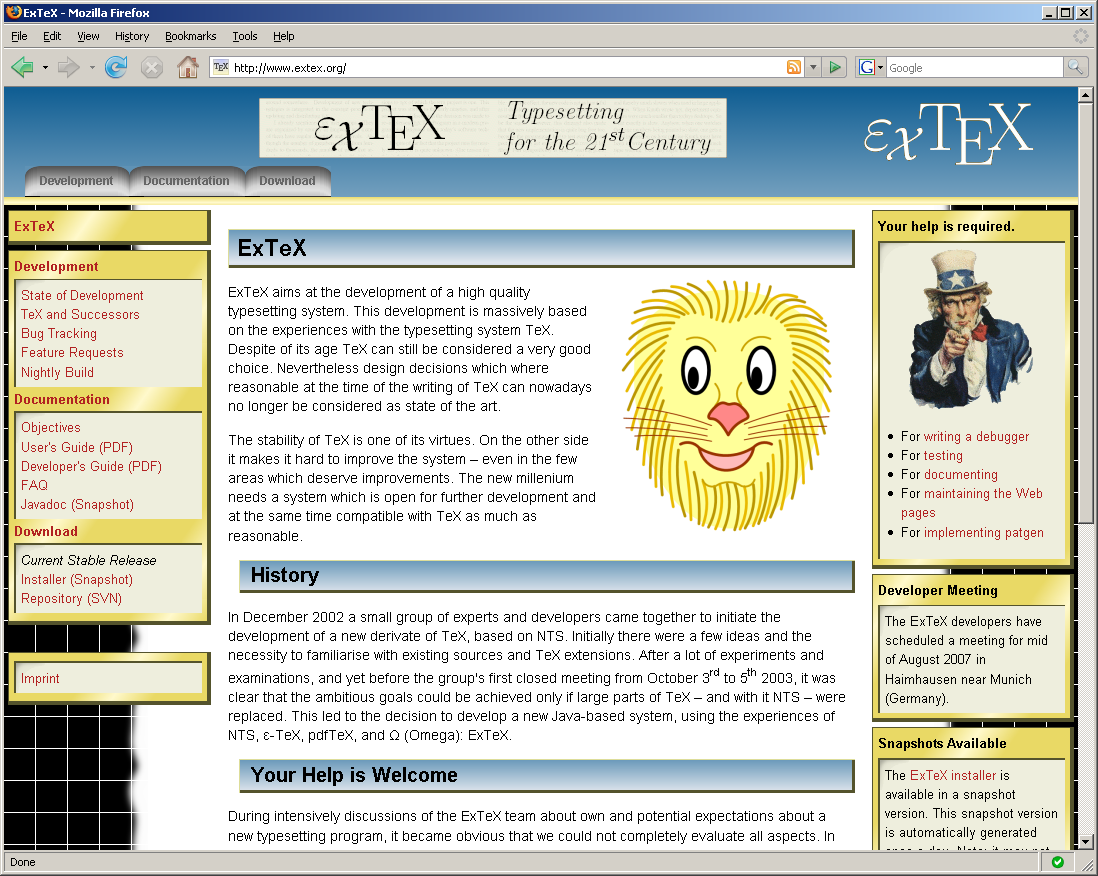
\includegraphics[width=.5\textwidth]{img/www-extex-org}
  \caption{\texttt{www.extex.org}}
  \label{fig:www.exetex.org}
\end{figure}
There is a web site devoted to \ExTeX.\index{WWW}\index{Web Site} This
web site (see figure~\ref{fig:www.exetex.org}) can be reached via the
URL\index{www.extex.org}
\begin{quotation}
  \url{http://www.extex.org}
\end{quotation}


\section{Mailing Lists}
%@author Gerd Neugebauer

If you are ready to try \ExBib{} you might as well want to join a
mailing list to get in contact with the community.\index{mailing list}

\begin{quotation}
  \url{http://www.dante.de/listman/extex}
\end{quotation}


\section{Reporting Bugs}
%@author Gerd Neugebauer


If you find any bugs in \ExBib\ you can submit them 
%either 
via a HTML form.
% or via email. 
You can find the HTML form at
\begin{quotation}
  \url{http://www.extex.org/bugs}
\end{quotation}
%Emails containing the description can be sent to
%\begin{quotation}
%  \href{mailto:extex-bugs@dante.de}{extex-bugs@dante.de}
%\end{quotation}

Please include in your description 
\begin{itemize}
\item the source of a \emph{minimal} example showing the problem
\item the log file resulting from running this example
\item a description why you think that something went wrong and what
  the expected result would be
\item a description of the environment you are using (host
  architecture, operating system, Java version)
\end{itemize}

\endinput
%
% Local Variables: 
% mode: latex
% TeX-master: "exbib-users"
% End: 
